\newpage
\chapter{Diseño de Prototipos}
\label{ch:capitulo4.tex}

\begin{FraseCelebre}

\begin{Frase}
		La cosa está muy mal... estoy friendo los huevos con saliva
	\end{Frase}
    
	\begin{Fuente}
	Gregorio Esteban Sánchez
	\end{Fuente}

\end{FraseCelebre}


En este capítulo se muestra el diseño de los distintos modelos que se han generado para el proyecto. Se dispone, para cada uno, una vista en 3D, creada con \textit{OpenScad}, que representa la disposición de los distintos componentes y la dirección de las corrientes de aire generadas por los ventiladores, finalmente, se incluyen capturas del resultado de cada uno de ellos.

\section{Características del modelado}
\label{makereference4.2}
\paragraph{}

Los componentes representados en el modelo en 3D son: el switch de ocho puertos (\textcolor[rgb]{0.16,0.3,0.67}{Azul}), un clúster de Raspberrys formado por siete nodos (\textcolor[rgb]{0.1,0.57,0.2}{Verde}), la base de enchufes (\textcolor[rgb]{0.71,0.28,0.25}{Rojo}) y los ventiladores (\textcolor[rgb]{0.58,0.58,0.58}{Gris}), no se incluyen los cables y conectores conectados a la base y a cada Raspberry.

En cuanto a la disposición de los ventiladores, para cada uno de los modelos, se han realizado diferentes configuraciones, todas ellas destinadas a obtener la corriente de aire más eficiente y la mejor tasa de temperatura cuando los nodos están trabajando a máximo rendimiento. 

Los resultados de estas se muestran en el capítulo \ref{ch:capitulo5.tex}, en donde se verá el comportamiento de cada una con una serie de pruebas destinadas a medir la temperatura ante distintos escenarios.

\section{Modelo 1} 
\label{makereference4.3}
\paragraph{}

En este modelo la distribución de aire se hace con los ventiladores opuestos entre sí, creando una corriente de aire alrededor del rack de Raspberrys que se encuentra frente a ellos. 
 
\begin{figure}[H]
	\centering
  	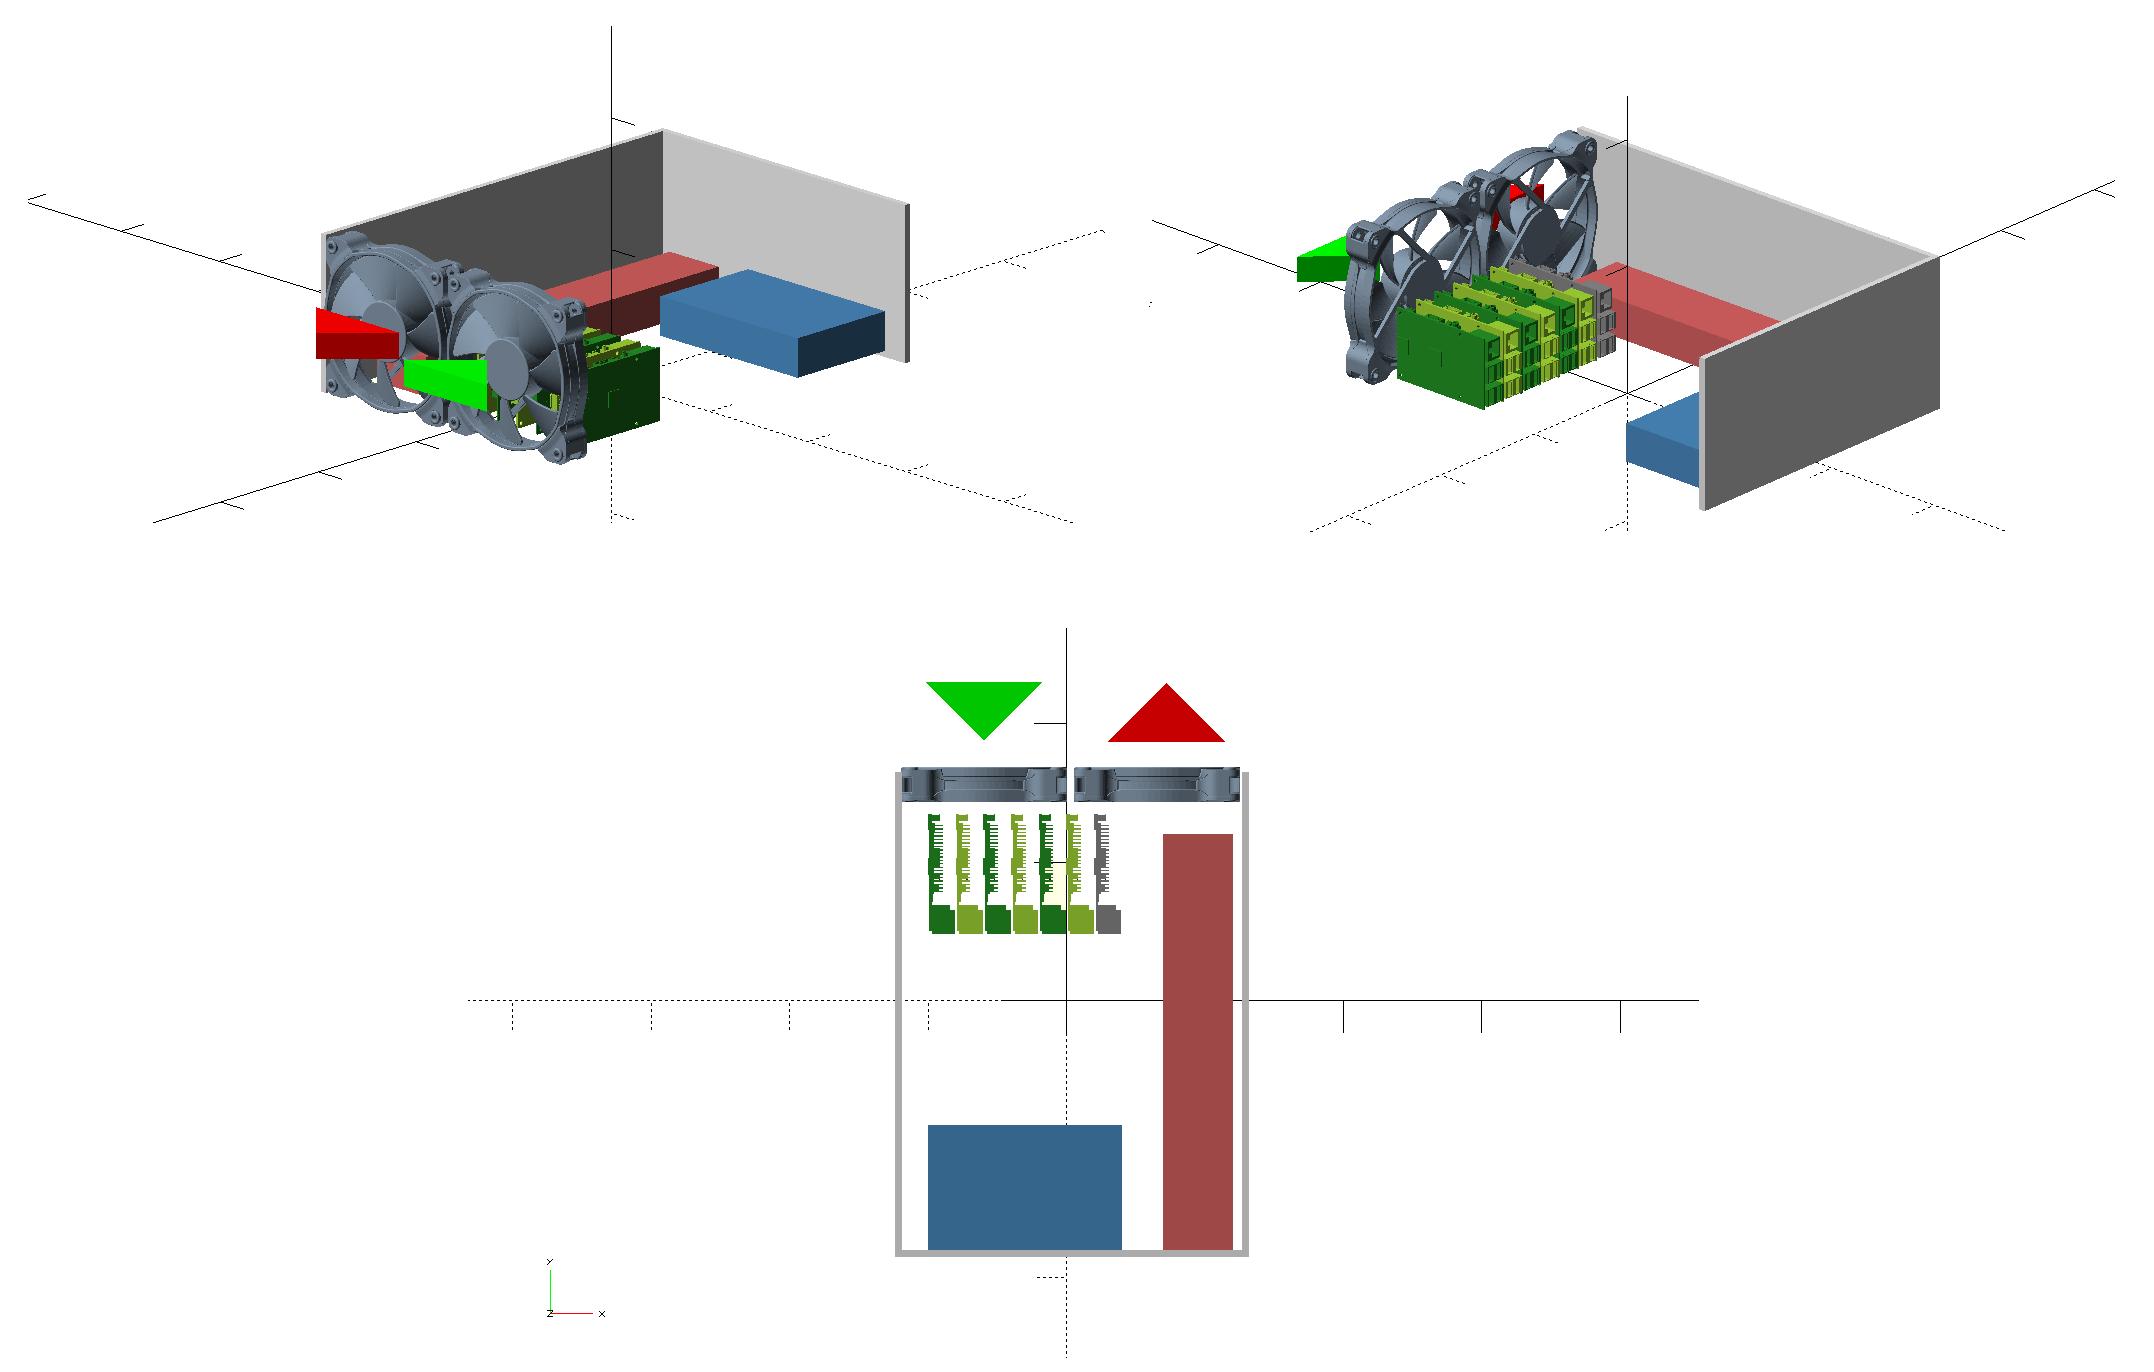
\includegraphics[width=120mm]{Modelos/M1X.png}
   	\caption[Modelo 1 3D]{Modelo 1 3D}
   \label{figure4.1}
\end{figure}

La figura \ref{figure4.1} muestra la vista trasera, delantera y alzada del modelo. La prioridad es obtener una buena distribución de aire, no se ha tenido en cuenta la facilidad para acceder a los componentes.
Para poder acceder a las tarjetas \textbf{SD} de cada Raspberry es necesario mover todo el rack, lo que hace que sea complicado, una solución alternativa sería ofrecer la opción de desacoplar uno de los ventiladores para facilitar el acceso.

\subsection{Resultado}
\paragraph{}

Este modelo tiene un tamaño de 122x123x35 cm y en la captura no se han incluído los cables rj45 que conectan el rack de Raspberrys con el switch.
Podemos observar que los componentes disponen de un espacio muy limitado y que la poca flexibilidad de los cables dificulta el cierre del contenedor.

\begin{figure}[H]
	\centering
  	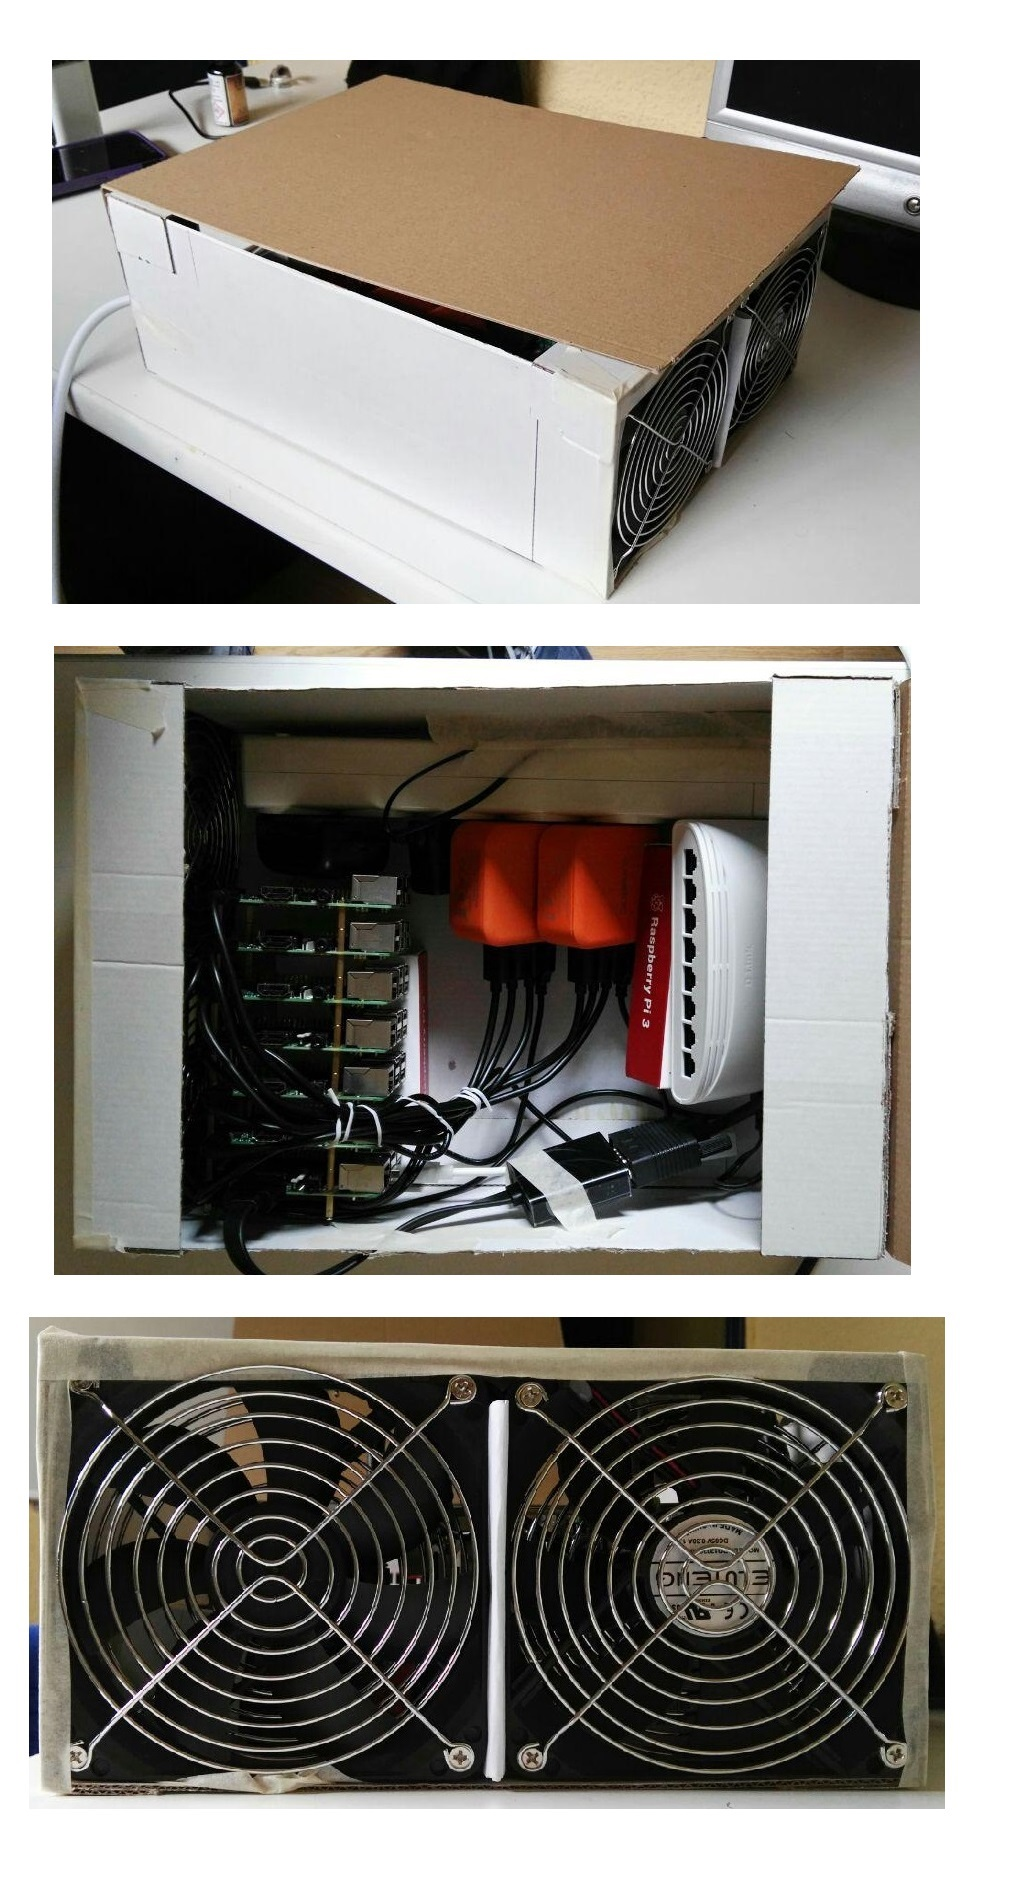
\includegraphics[width=60mm]{Modelos/M1Res.jpg}
   	\caption[Resultado Modelo 1]{Resultado Modelo 1}
   \label{figure4.2}
\end{figure}

Las figura \ref{figure4.2} muestra el resultado del diseño descrito en el apartado anterior, se puede observar la distribución de los componentes dentro del contenedor y el cierre del que dispone.

\section{Modelo 2}
\label{makereference4.4}
\paragraph{}

Para resolver los problemas de accesibilidad al rack este modelo dispone de una apertura lateral que expone las tarjetas \textbf{SD} de cada Raspberry, con lo que no es necesario abrir el contenedor para extraer cada tarjeta.
Además el contenedor está dividido en dos piezas, una que se acopla sobre la otra para formar un cubo, esto facilita la apertura y acceso al mismo.

\begin{figure}[H]
	\centering
  	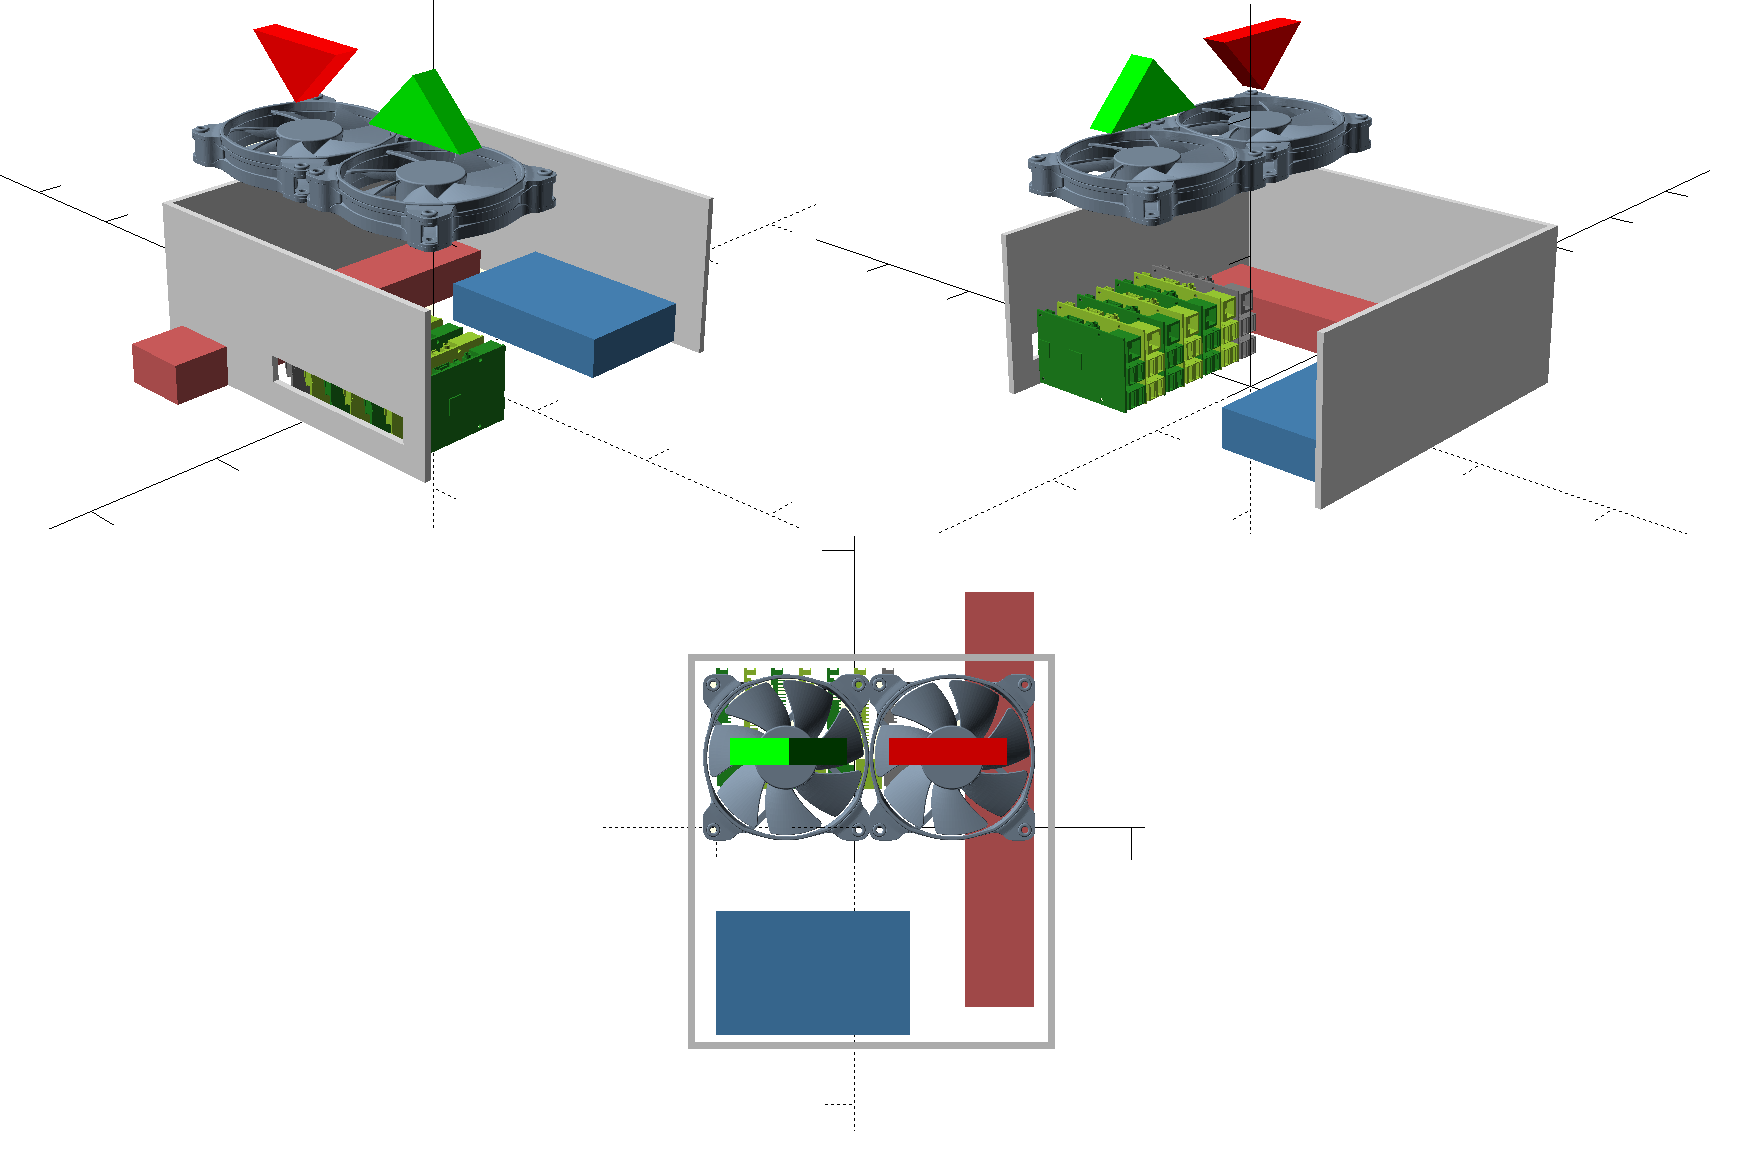
\includegraphics[width=120mm]{Modelos/M2X.png}
   	\caption[Modelo 2 3D]{Modelo 2 3D}
   \label{figure4.3}
\end{figure}

Como se muestra en la figura \ref{figure4.3} la ventilación se realiza desde la parte superior, creando, como en el caso anterior, una corriente de aire debida al emplazamiento de cada ventilador. Se puede observar, en la vista frontal, la apertura centrada sobre el rack de Raspberrys.
Este modelo es más compacto que el anterior, parte de la base de enchufes queda en el exterior. Sin embargo, existe un mayor espacio entre los ventiladores y el rack.
La disposición de los cables de alimentación del rack es mejor que la del modelo 1, junto con el acceso lateral, prácticamente no es necesario manipular ninguno de los componentes.

\subsection{Resultado}
\paragraph{}

Este modelo tiene un tamaño de 122x123x35 cm, en la figura \ref{figure4.4} se puede observar el sistema de acople en dos piezas que abren el contenedor. Como se ha comentado anteriormente, parte de la base de enchufes queda en el exterior, esto supone una mejora ya que permite el encendido y apagado del clúster sin que sea necesario abrir todo el contenedor para ello. 

\begin{figure}[H]
	\centering
  	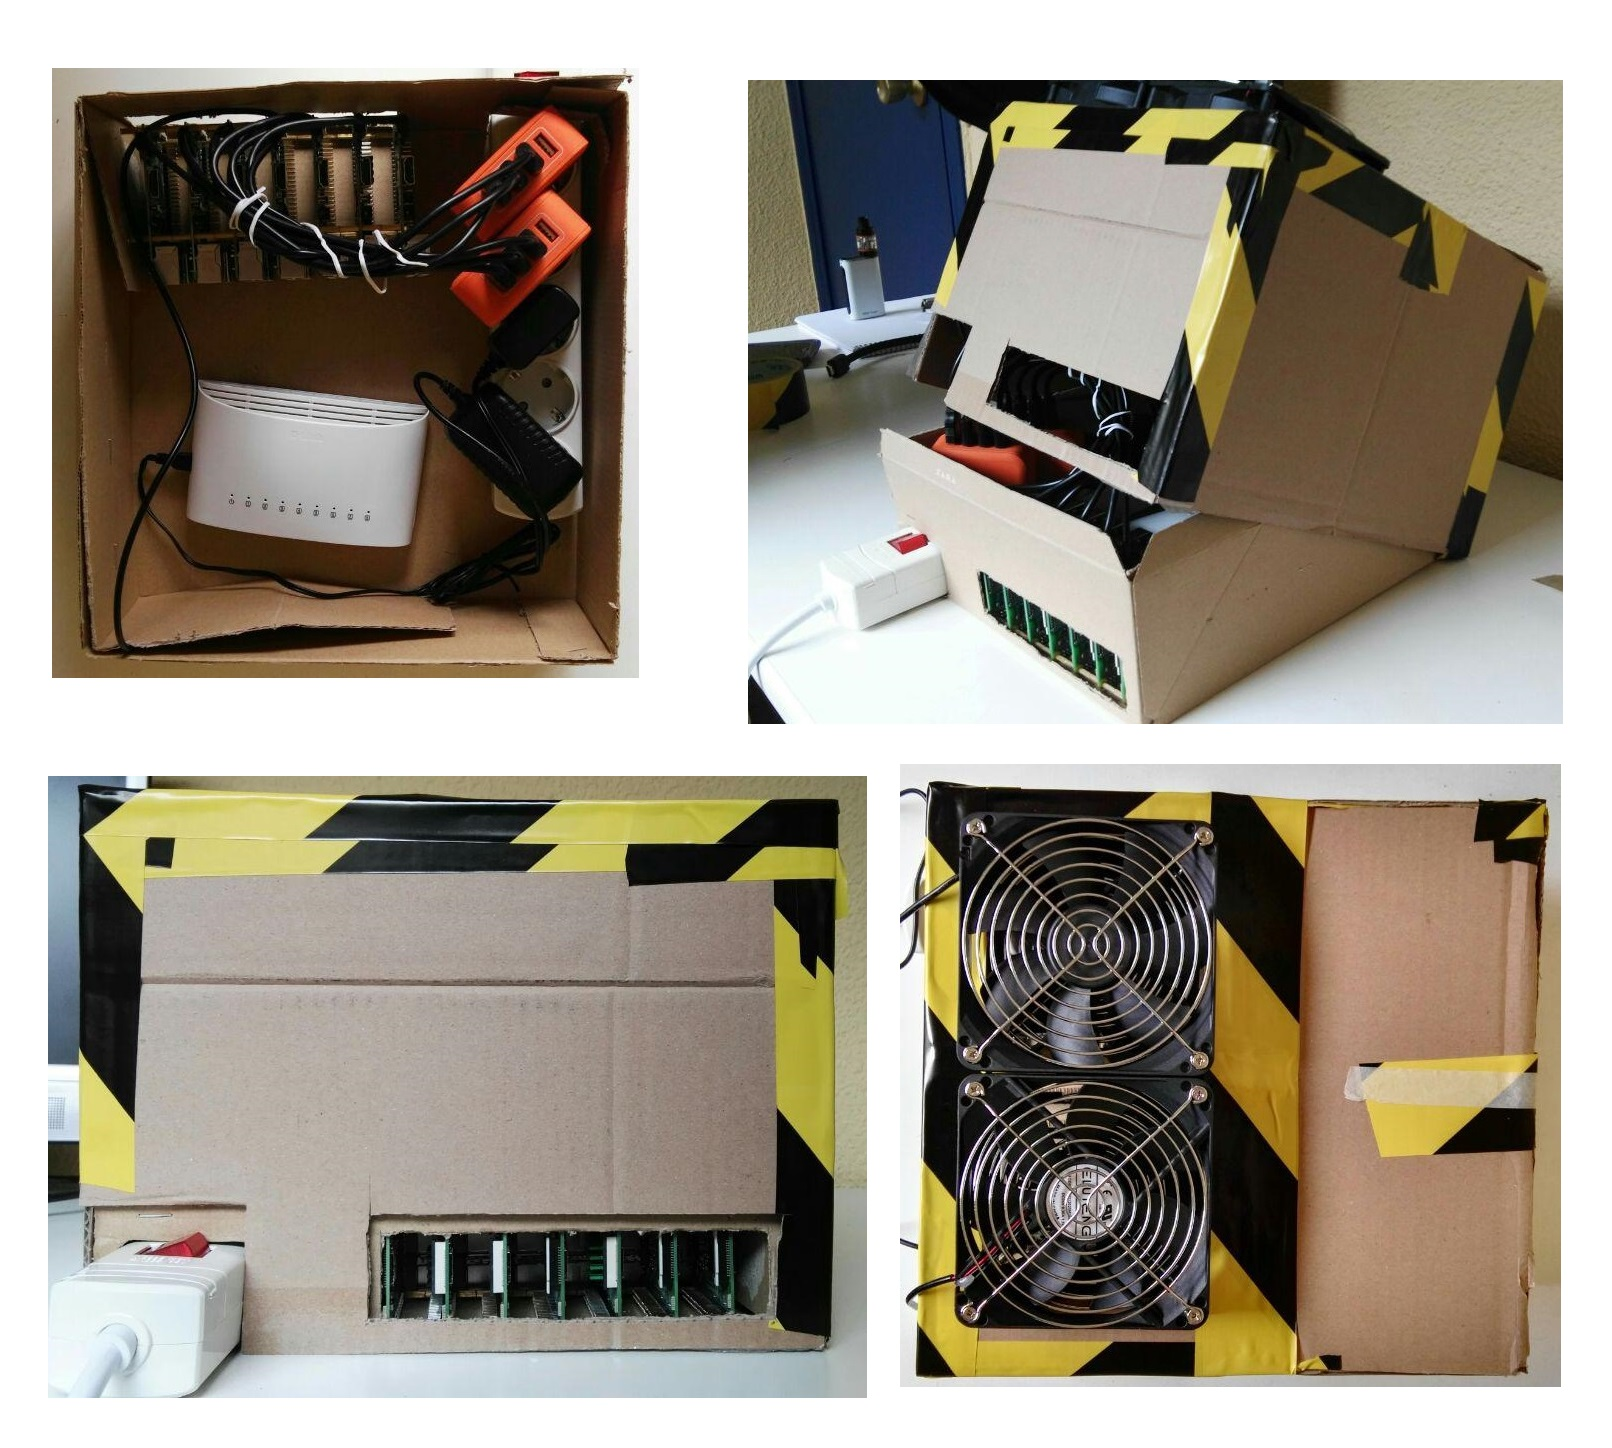
\includegraphics[width=100mm]{Modelos/M2Res.jpg}
   	\caption[Resultado Modelo 2]{Resultado Modelo 2}
   \label{figure4.4}
\end{figure}

Como resultado de todas estas mejoras tenemos un modelo que es mucho mas manejable que el anterior, de tamaño más reducido y con mejoras estructurales que facilitan la manipulación.

\section{Modelo 2b}
\label{makereference4.5}
\paragraph{}

El modelo 2b presenta unas modificaciones estructurales internas, tras hacer un estudio previo sobre corrientes de aire decidimos realizar algunas modificaciones sobre éste para conseguir mejorar la eficiencia del flujo de aire dentro del contenedor.

\begin{figure}[H]
	\centering
  	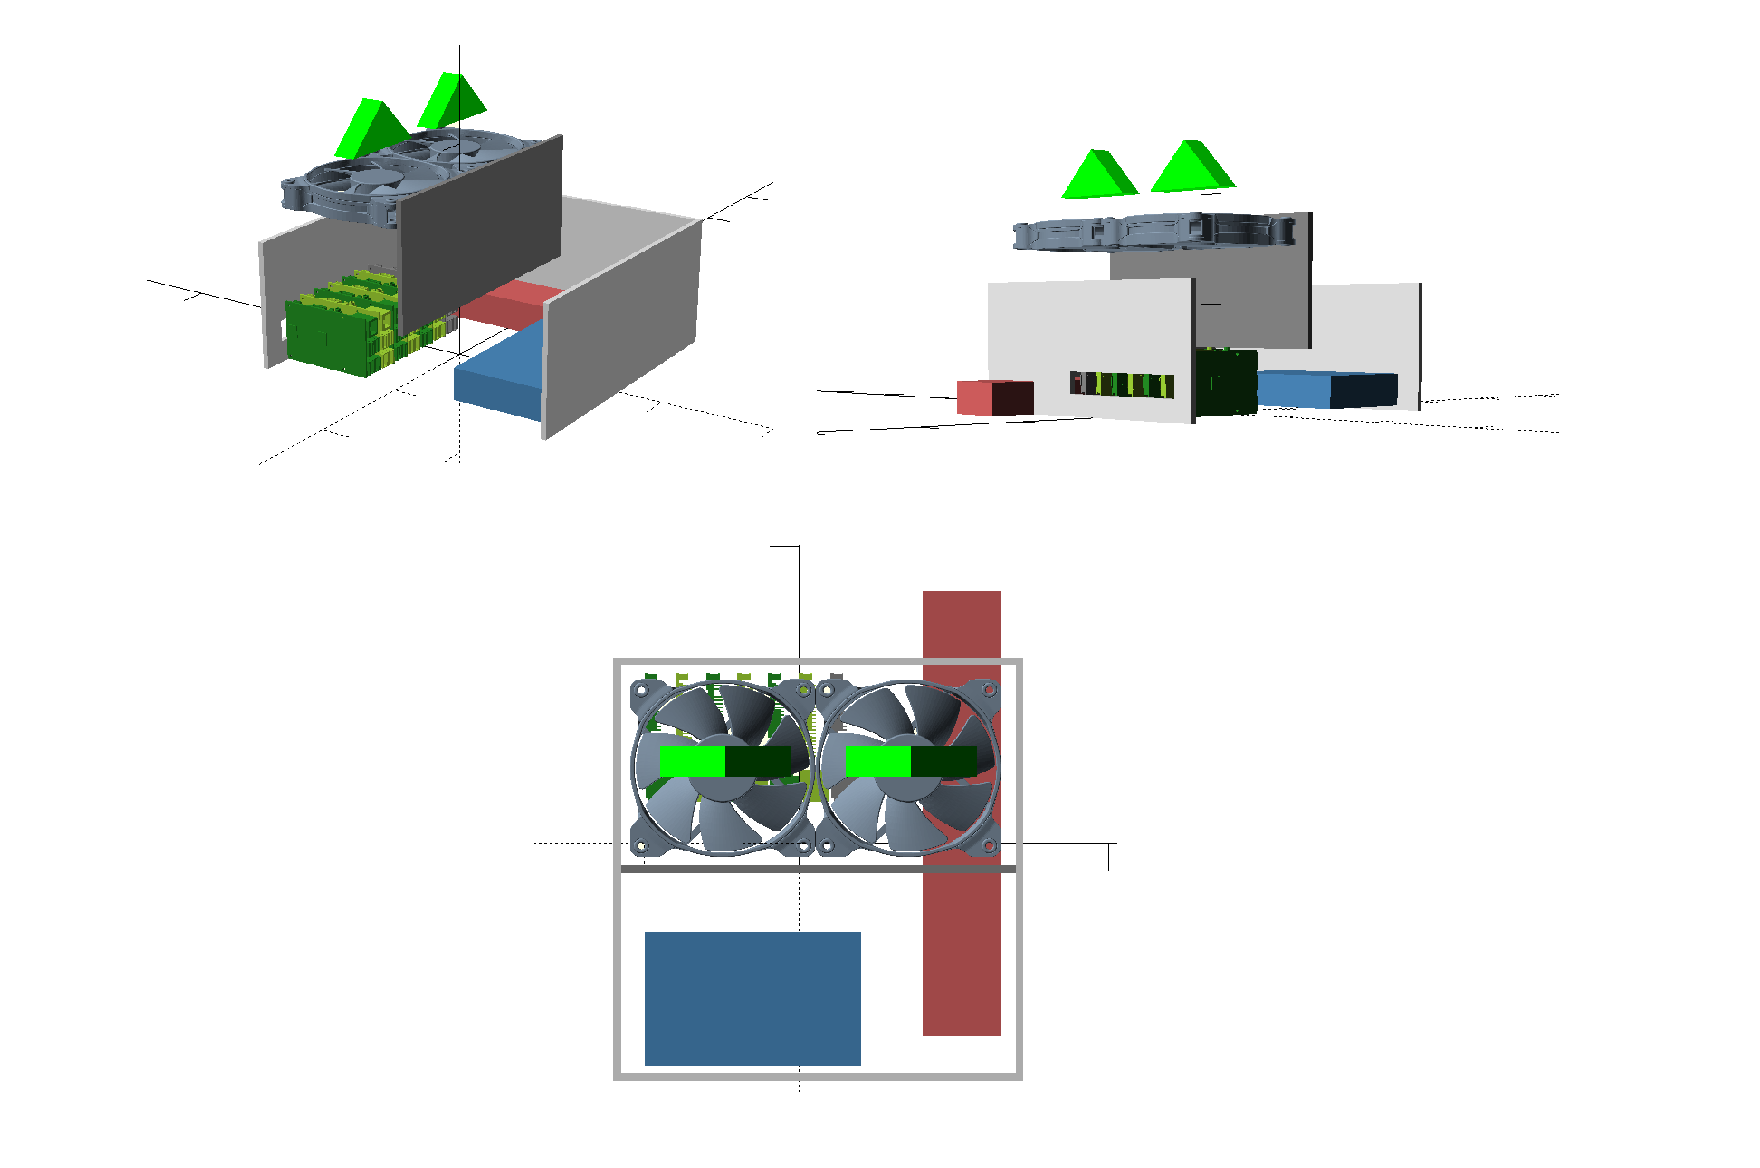
\includegraphics[width=120mm]{Modelos/M2bX.png}
   	\caption[Modelo 2b 3D]{Modelo 2b 3D}
   \label{figure4.5}
\end{figure}

Para esto, se incluye una nueva pared interior, distribuyendo el contenedor en \textit{dos cámaras}, una que contiene el rack de Raspberrys y otra con el switch. La corriente de aire se concentra en la primera cámara, con esto generamos un flujo que entra en el contenedor a través de la entrada lateral, en la que están expuestas las Raspberrys, pasando por cada uno de los procesadores y saliendo por la parte superior en la que ambos ventiladores expulsan el aire.

La figura \ref{figure4.5}, similar a la del modelo 2, muestra la separación en cámaras y distribución de los ventiladores.
Como se puede comprobar en el capítulo \ref{ch:capitulo5.tex} esta modificación ofrece unos resultados completamente distintos en cuanto a las temperaturas del contenedor.


\section{Modelo 3}
\label{makereference4.6}
\paragraph{}

Hemos diseñado el modelo 3 utilizando la arquitectura de \textit{túnel de viento}, éste consiste en suministrar una corriente de aire de entrada sobre las partes que más tienden a calentarse, en este caso, el rack de Raspberrys, aplicando una corriente de succión con un ventilador de salida, creando un flujo de aire horizontal. 
 
\subsection{Modelado 3D}
\paragraph{}

\begin{figure}[H]
	\centering
  	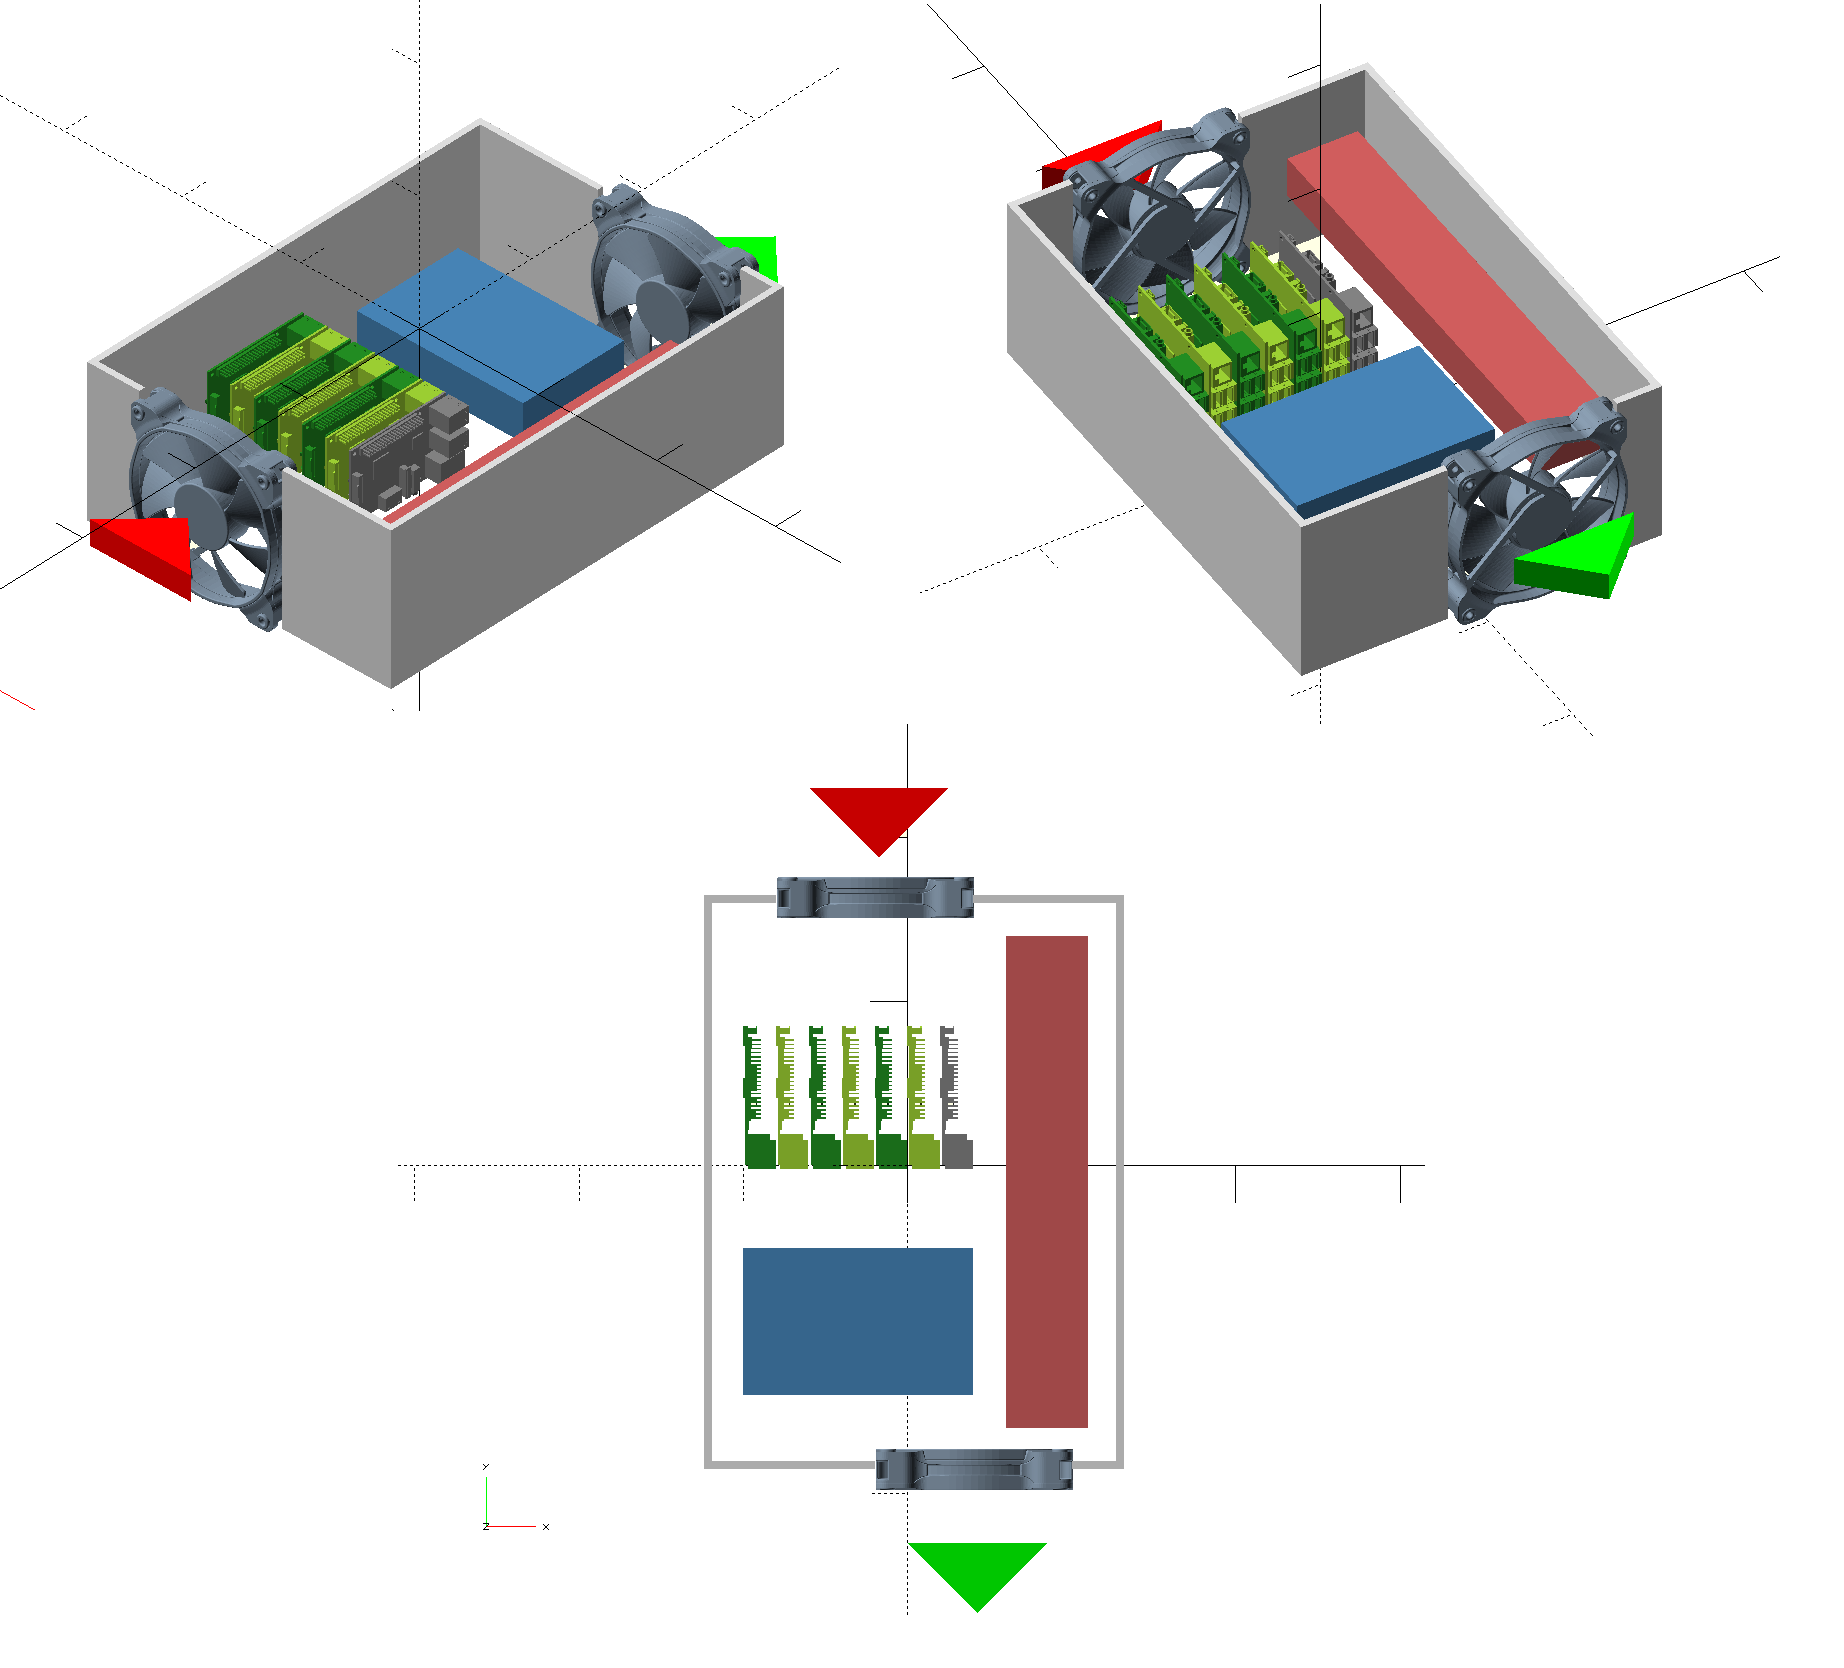
\includegraphics[width=100mm]{Modelos/M3X.png}
   	\caption[Modelo Modelo 3 3D]{Modelo 3 3D}
   \label{figure4.6}
\end{figure}

Debido a las altas temperaturas presentadas por el modelo 1 decidimos aplicar una corriente de aire directa sobre las Raspberrys y sacarla del sistema para evitar bucles de aire calientes a través del segundo ventilador que está situado al lado del switch como se muestra en la figura \ref{figure4.6} 

Tras una serie de pruebas y mediciones de temperatura con la disposición de los ventiladores, entrada-salida, entrada-entrada y salida-salida, llegamos a la conclusión que la más eficiente era la primera de ellas.

\subsection{Resultado}
\paragraph{}

Tras el desarrollo de los modelos anteriores, hemos creado un híbrido entre el modelo 1 y 2B, del primero aprovechamos su base y el ventilador del que ya disponíamos, del segundo, hemos decidido que en vez de aplicar la corriente de succión en la parte de arriba, le otorgaremos un flujo de aire que recorre todo el contenedor a través del túnel de viento ya mencionado. Mientras los anteriores modelos se centraban en las Raspberrys, este proporciona una corriente tanto al Switch como al rack. 

\begin{figure}[H]
	\centering
  	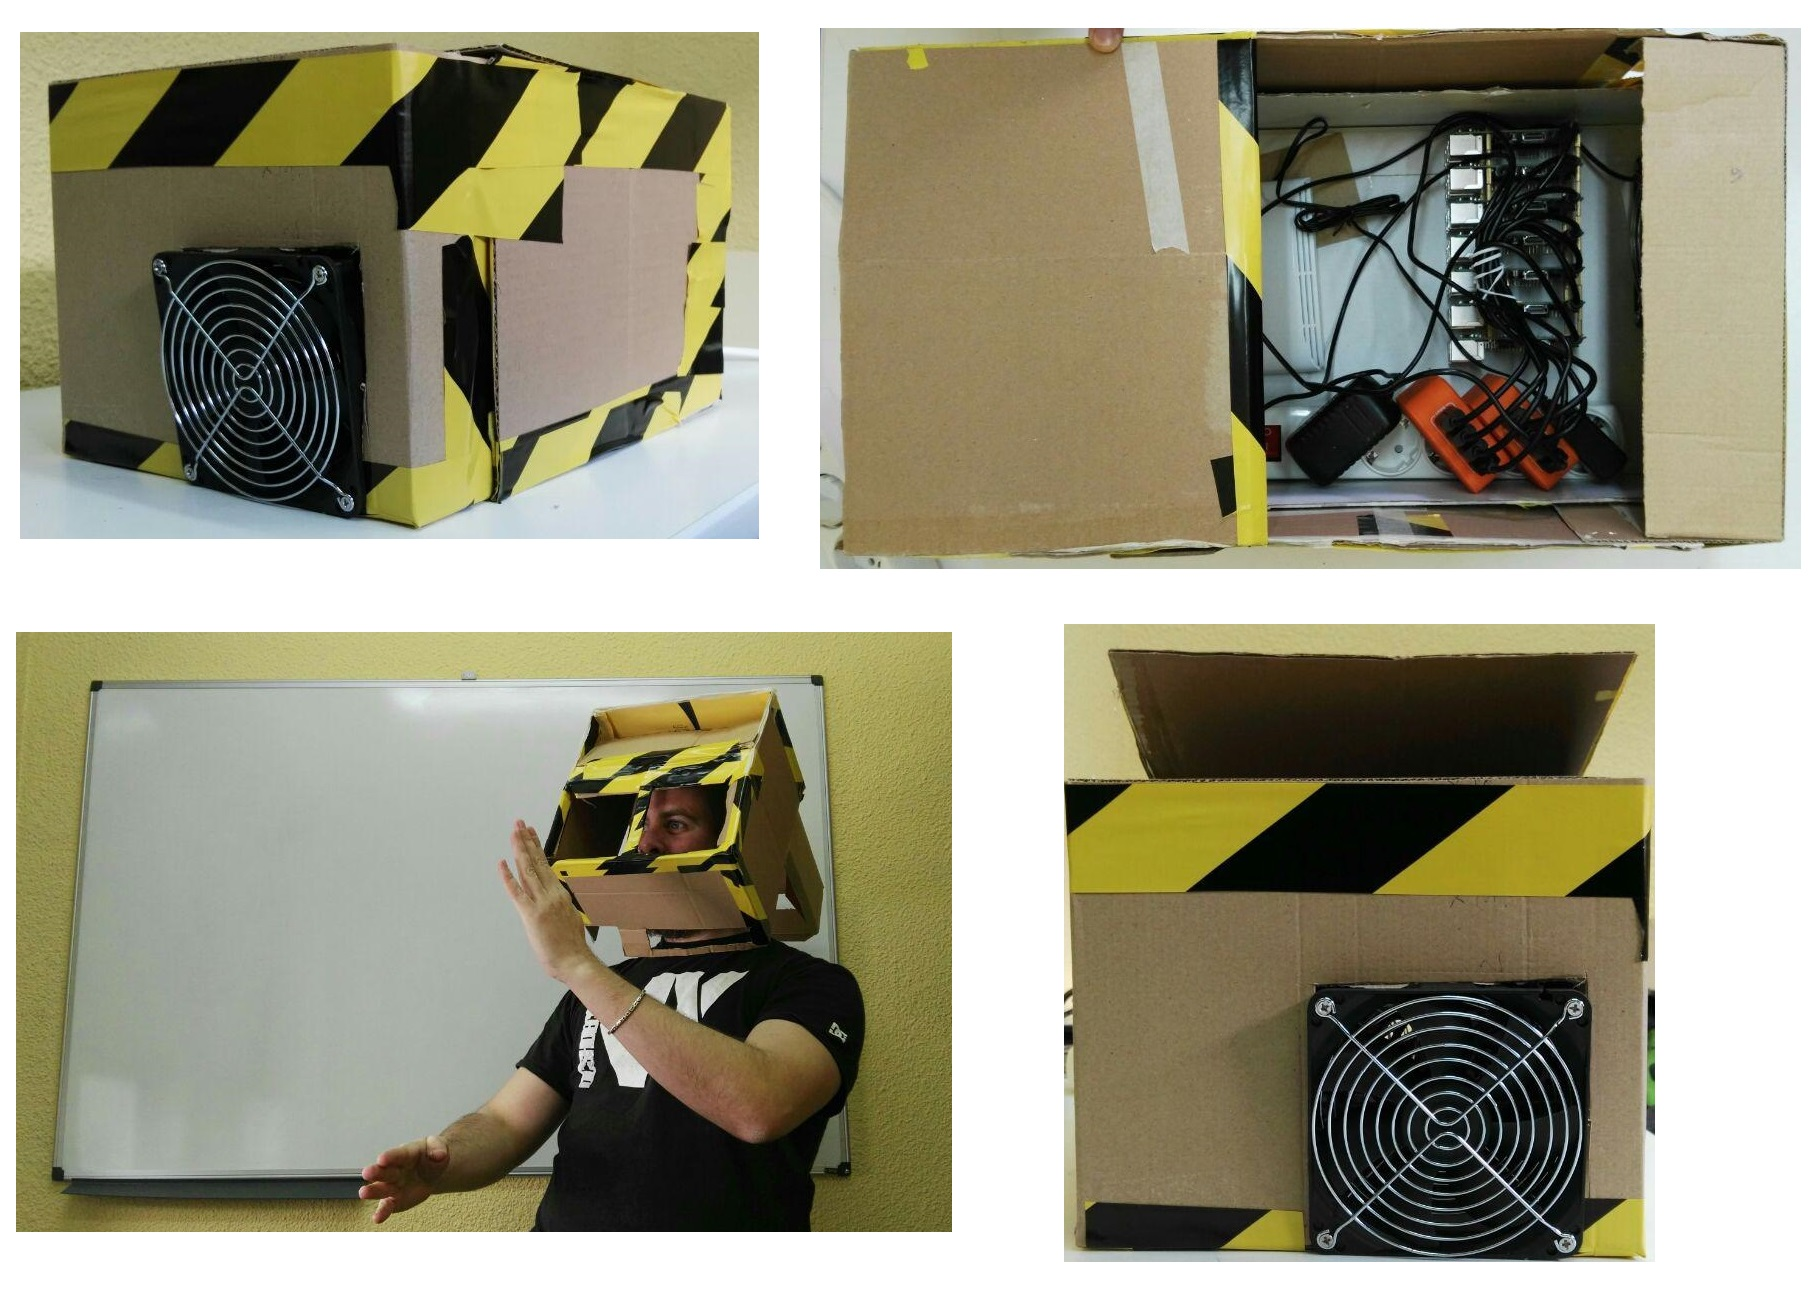
\includegraphics[width=100mm]{Modelos/M3Res.jpg}
   	\caption[Resultado Modelo 3]{Resultado Modelo 3}
   \label{figure4.7}
\end{figure}

El T-800 de la figura \ref{figure4.7} no está incluido en el pack, presentó demasiadas complicaciones a nivel de diseño y entraba continuamente en conflicto debido a las tres leyes de la robótica.
